MiniTwit follows the server-client architecture, and the server is deployed via a Docker Swarm, which consists of virtual machines (aka 'droplets') on DigitalOcean. Data, such as user-data, messages and followers are stored in a PostgreSQL database, which is also hosted on DigitalOcean. \\
In the swarm, we have manager-nodes and worker-nodes. The only services allowed to run on the managers are Prometheus and Dozzle (more about the swarm services in section 4). Figure \ref{fig:DeployDiagram} is a Specification Level Deployment Diagram, which shows how ITU-MiniTwit is deployed on a worker-node.
\begin{figure}[h]
\centering
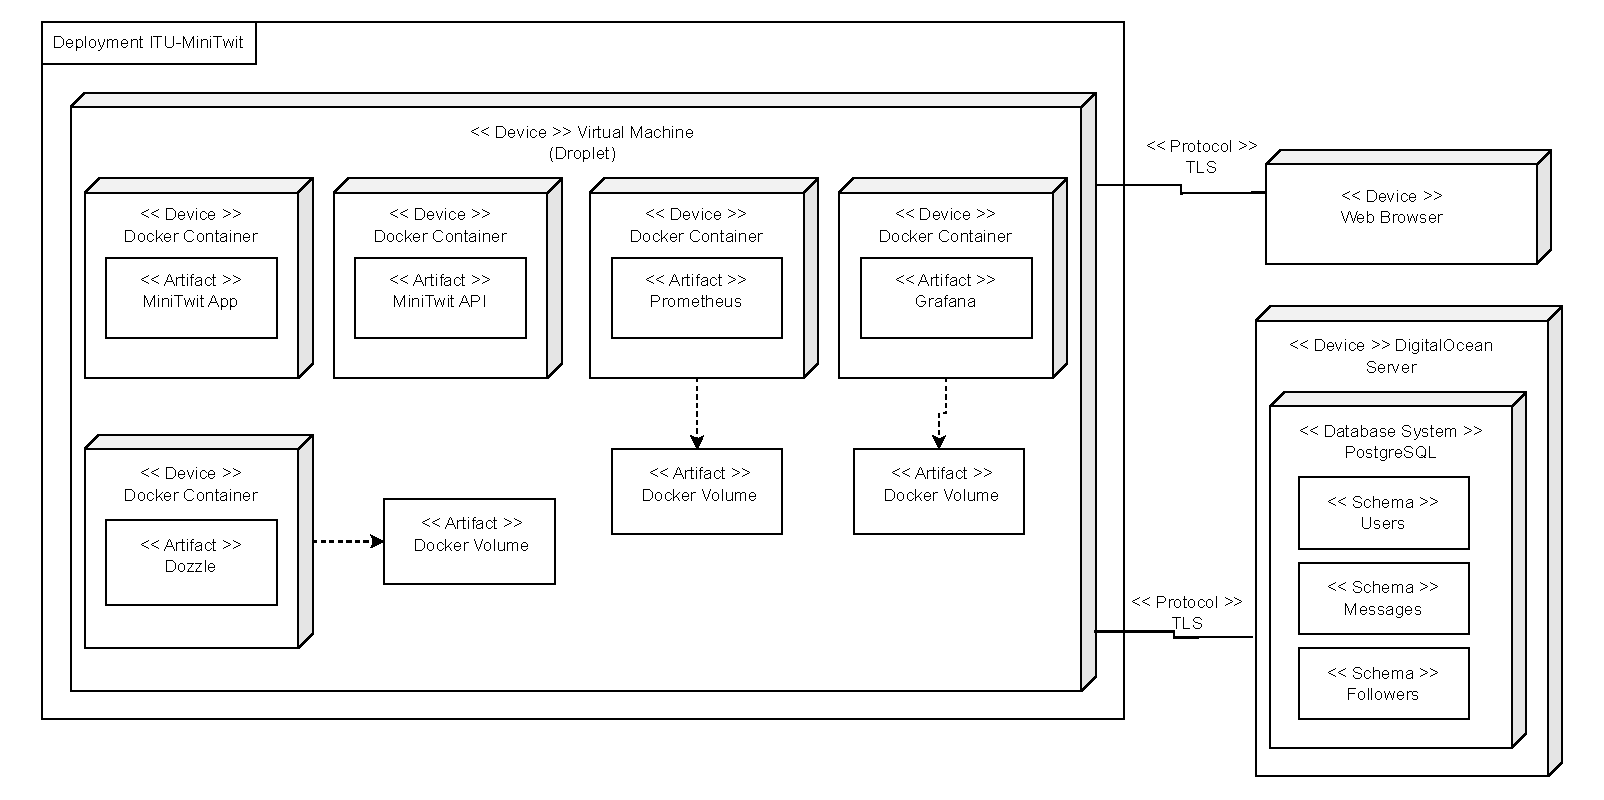
\includegraphics[width=\textwidth]{images/DeployDiagramWIP.pdf}
\caption{WIIIP}
\label{fig:DeployDiagram}
\end{figure}